\begin{figure}[t]
	\vspace{-0.75em}
	\centering
	\begin{tabular}{cc}
		\hspace{-0.95em}\subfloat[][{\sf intel}]{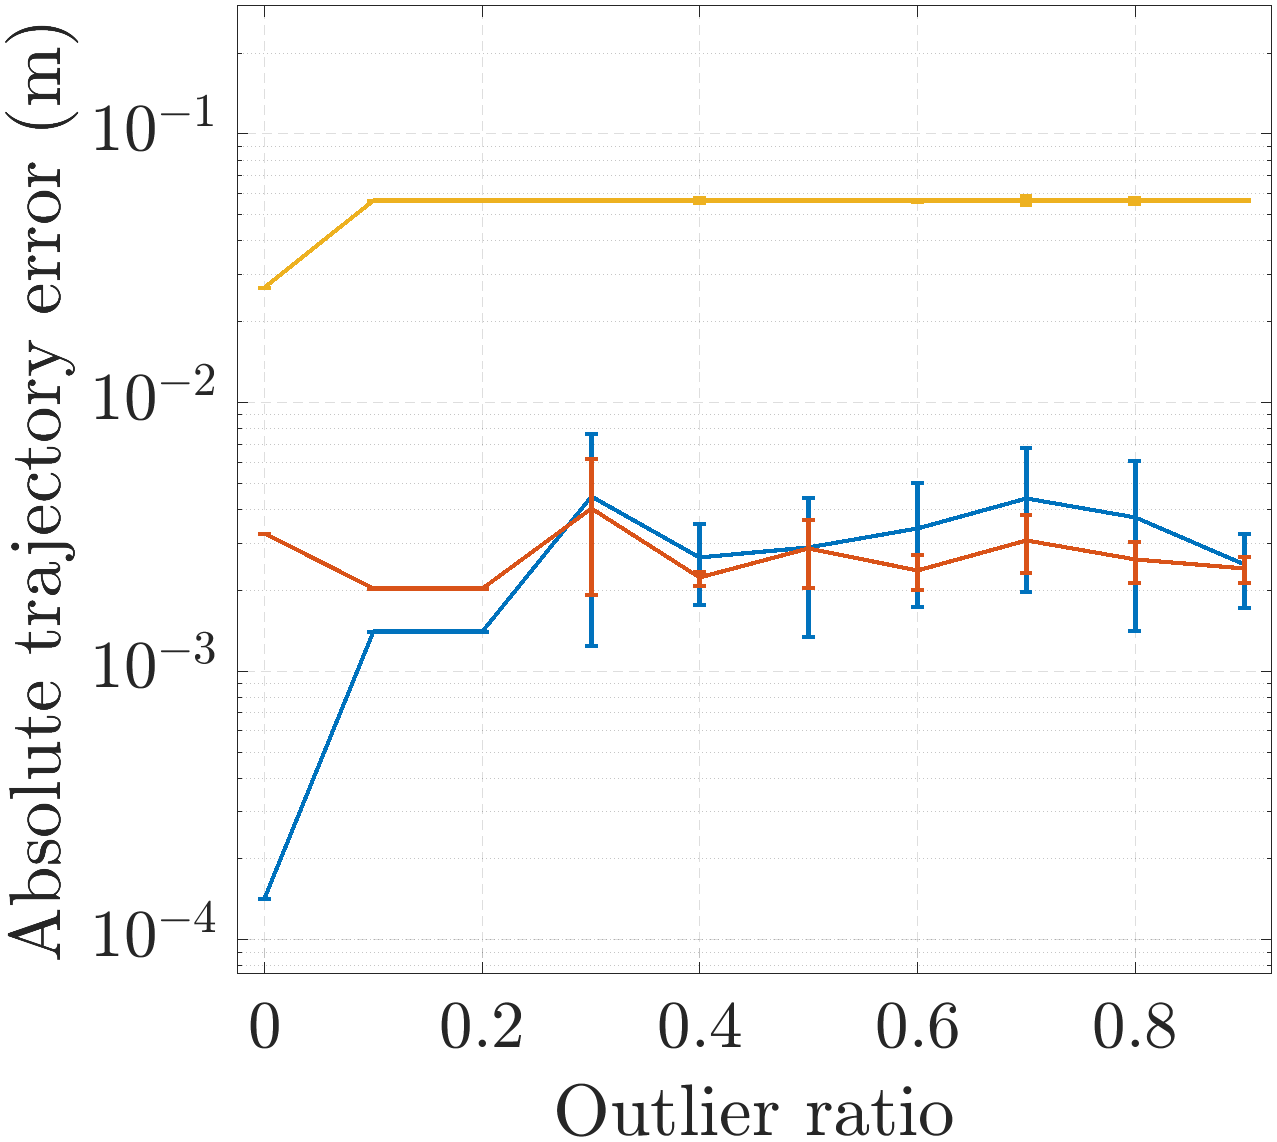
\includegraphics[trim =0mm 0mm 0mm 0mm,width=0.235\textwidth]{figures/outlier/ate_outlier_intel.png}} &
		\hspace{-0.55em}\subfloat[][{\sf garage}]{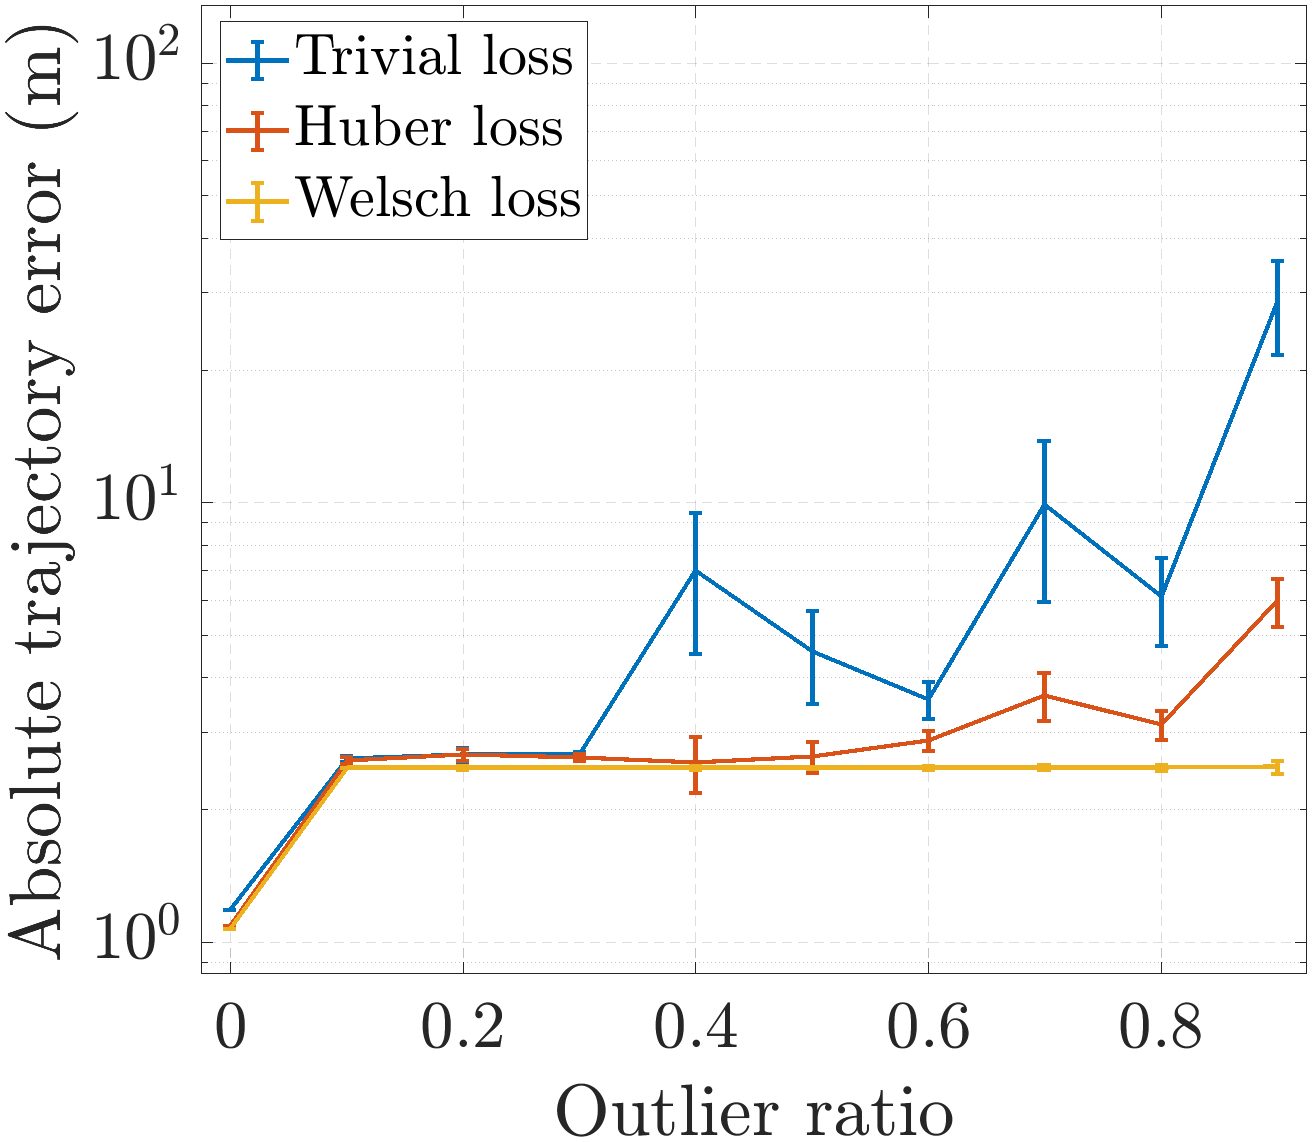
\includegraphics[trim =0mm 0mm 0mm 0mm,width=0.2425\textwidth]{figures/outlier/ate_outlier_garage.png}}
	\end{tabular}
	\caption{Absolute trajectory errors (ATE) of distributed PGO using $\ammd$ with the trivial, Huber and Welsch loss kernels on the 2D {\sf intel} and 3D {\sf garage} datasets.  The {\highlight outlier ratios} of inter-node loop closures are $0\sim 0.9$. The ATEs are computed against the outlier-free results of $\sesync$ \cite{rosen2016se} and  are averaged over $10$ Monte Carlo runs.   $\pcm$  \cite{mangelson2018pairwise} is used to initially reject spurious loop closures.   }\label{fig::outlier}
	\vspace{-.5em}
\end{figure}